\section{Results}
\label{sec:results}
In this section, we highlight the most notable descriptive statistics and statistically significant findings. A detailed summary of the outcomes for each quantitative, comparative survey question is provided in the Appendix.

In instances where survey questions covered multiple key performance indicators (KPIs), the findings are presented across multiple subsections. This approach ensures that each KPI is thoroughly addressed and the results are clearly communicated in their respective areas of relevance.

For the paired testing, which compared pre-connection data to post-connection data in that order, a negative result indicates a decrease over time while a positive result signifies an increase. 

In this section, where applicable, 95\% confidence intervals for a result are denoted using the "$\pm$" symbol (e.g., $10\pm1$).

\subsection{Survey Distribution}
\begin{figure}[th]
    \centering
    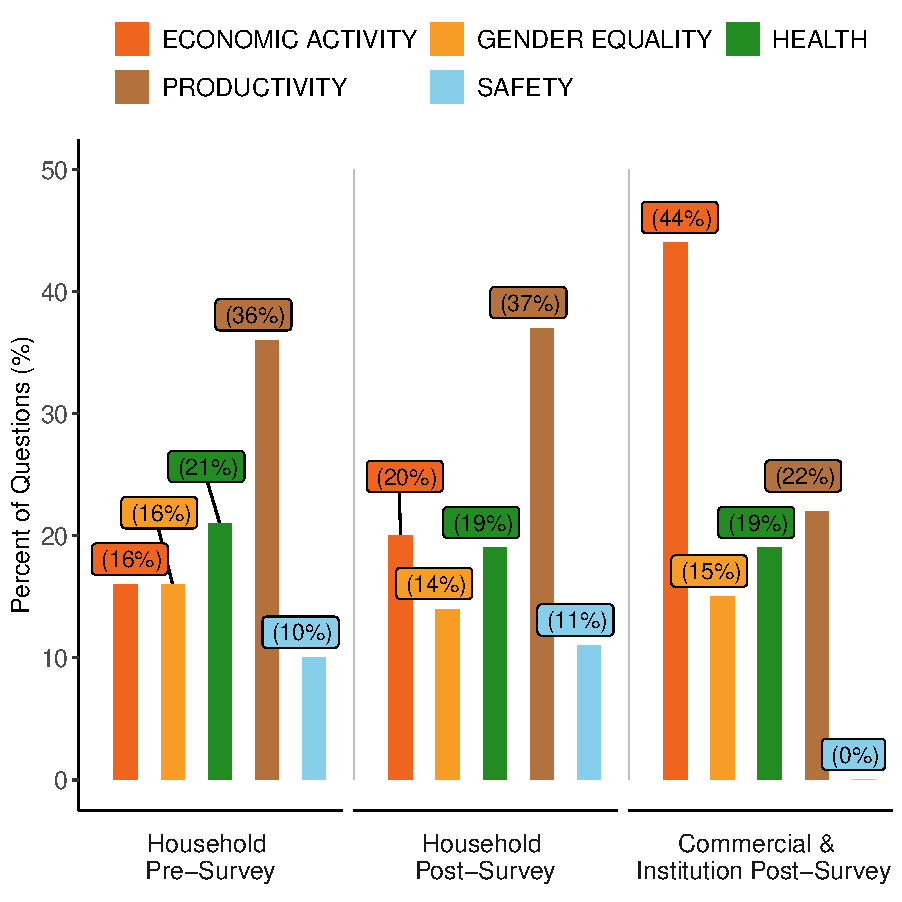
\includegraphics[width=0.8\textwidth]{images/questions_distribution_plot.pdf}
    \caption{Distribution of Survey Questions}
    \label{fig:distrbution_questions}
\end{figure}

There are a total of 86 questions for the pre-connection household survey and 93 and 37 for the post-connection household and organizational surveys, respectively. The pre- and post-connection household surveys shared 64 questions, thus enabling direct comparison of individual customer responses before and after connection. The questions were distributed among the five KPIs according to \cref{fig:distrbution_questions}. Correlation tables detailing the responses to the survey questions are presented in \cref{fig:corr-pre,,fig:corr-post-hh,,fig:corr-post-ci} in the appendix.

\subsection{Characteristics of the Respondents}
Out of the 3,952 total responses from the initial survey, 564 distinct households (14.3\%) were retained for analysis. To isolate the sample from pre-connection households, the remainder of observations at post-connection and duplicate responses were excluded. At post-connection, 2,202 responses were retained from the 2,603 (84.6\%) total responses collected after a similar data validation process. From the pre and post samples, 468 respondents could be paired. The high turnover rate is mainly due to the nomadic or otherwise transitory nature of the communities surveyed.

% \begin{figure}[th]
%     \centering
%     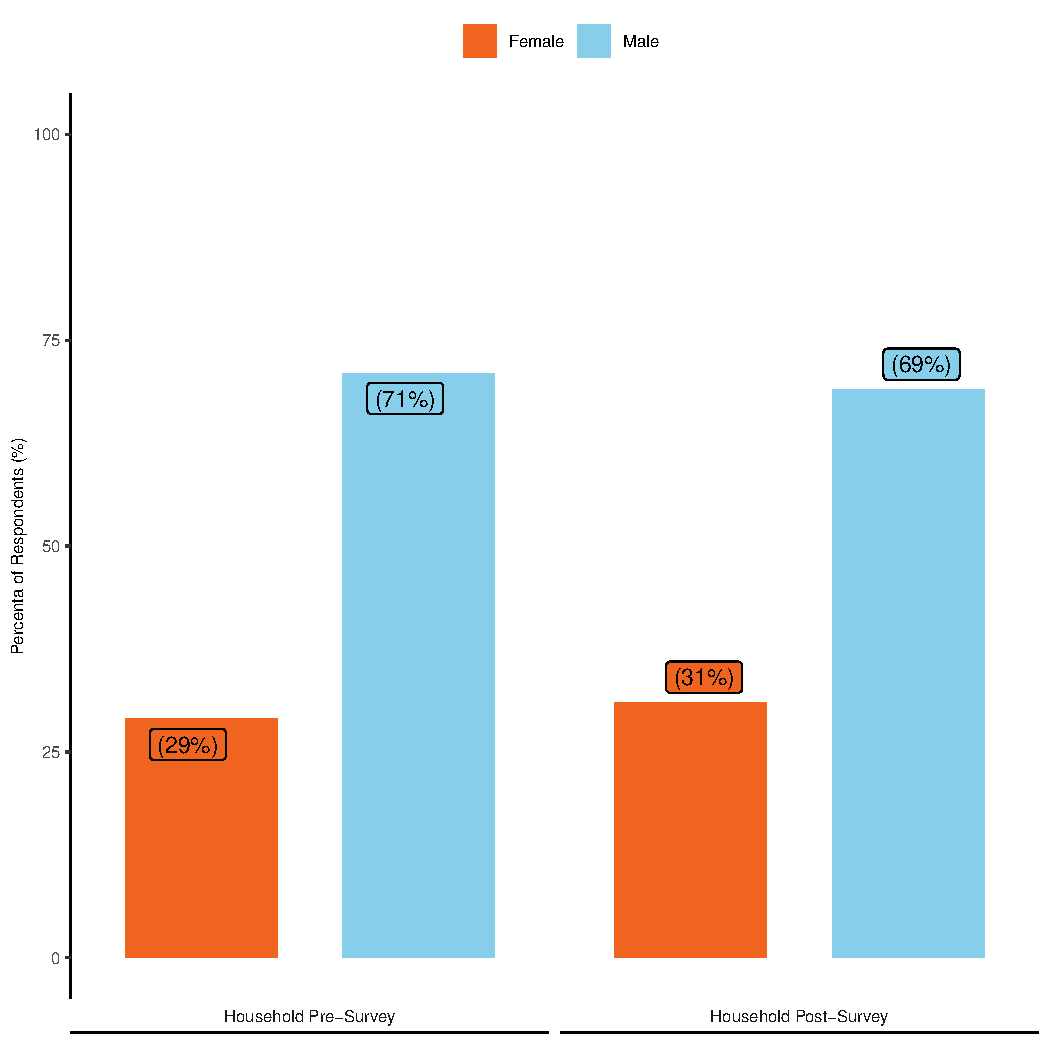
\includegraphics[width=0.7\textwidth]{images/gender_distribution_plot.pdf}
%     \caption{Gender Distribution of Respondents}
%     \label{fig:dsitrbution_gender}
% \end{figure}

\begin{table}[th]
\centering
    \begin{tabular}{*5c} 
        \toprule
        Variables &  & Statistic  &\multicolumn{2}{c}{Total}\\
        & &  & Pre-connection & Post-connection\\
        
        \midrule
        Sample Households  & & Count & 564 & 2202 \\
        Gender  & Male & Count & 400 & 1518\\
                & Female & Count & 164 & 678\\
                & Unidentified & Count & - & 6\\
        Age  &  & Median & 41 & 38\\
        Household Size  &  & Median & 6 & - \\
        Employment & Seasonal & Count & 360 & - \\
                   & Regular & Count & 139 & - \\
                   & Unemployed & Count & 60 & - \\
                   & Unidentified & Count & 5 & -\\
                   
        \bottomrule
    \end{tabular}
\caption{Descriptive Statistics of Households}
\label{tab:desc-stats-hh}
\end{table}

A demographic overview of the household respondents is presented in \cref{tab:desc-stats-hh}. Heads of household were responsible for responding to the survey, and the distribution based on gender shows a predominance of male respondents, with men making up 71\% of the pre-connection sample and 69\% of post-connection sample. The median age of the respondents was 41 and 38 years old for the pre- and post-survey, respectively. Before connection to the mini-grid, the median household had six members, and the breakdown of respondents' employment types was as follows: 64\% were seasonally employed, 25\% had regular employment, and 11\% were unemployed.

\begin{table}[th]
\centering
\begin{tabular}{*4c} 
    \toprule
    Variables &  & Statistic &  Post-Connection\\
    \midrule                 
    Sample Organizations  & & Count & 465 \\
    Status & In Operation & Count & 449 \\
           & Closed & Count & 7 \\
           & Unidentified & Count & 9 \\
    Organization Type  & Business & Count & 340 \\
                       & School & Count & 36 \\
                       & Clinic & Count & 22 \\
                       & Religious and Institution & Count & 67 \\
                       % & Miscellaneous & Count & 70\\
    \bottomrule
    \end{tabular}
\caption{Descriptive Statistics of Commercial and Institutional Customers}
\label{tab:desc-stats-com}
\end{table}

Out of the 470 total commercial and institutional responses from the initial survey, 465 distinct entities (99\%) were retained for further analysis. The remainder of duplicates and unidentifiable respondents were excluded. An overview of the socio-economic status of commercial and institutional customers is presented in \cref{tab:desc-stats-com}. The distribution based on organization type was broken down with 340 (73\%) businesses, 36 (8\%) schools, 22 (5\%) clinics, and 67 (14\%) religious institutions.
%, and 70 (15.4\%) miscellaneous organizations.

\subsection{Gender Equality}
% school
\begin{figure}[b]
    \centering
    \begin{subfigure}[t]{0.48\textwidth}
        \centering
        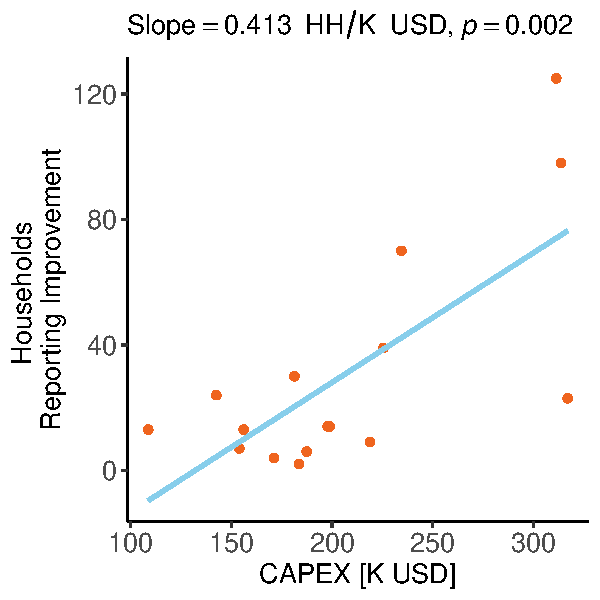
\includegraphics[width=\textwidth]{images/girls_schooling_change_regression_community.pdf}
        \caption{An additional \$50,000 CAPEX investment correlated with an additional 20 households reporting an increase in the number of girls attending school.}
        \label{fig:girls-school}
    \end{subfigure}
    \hfill
    \begin{subfigure}[t]{0.48\textwidth}
        \centering
        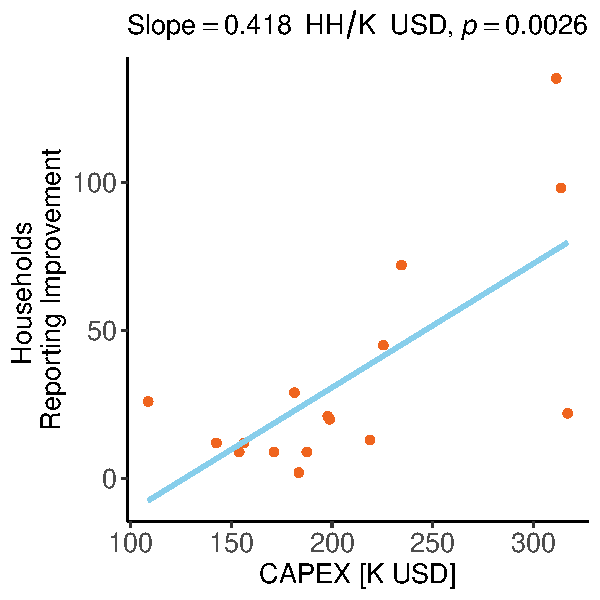
\includegraphics[width=\textwidth]{images/boys_schooling_change_regression_community.pdf}
        \caption{An additional \$50,000 CAPEX investment correlated with an additional 21 households reporting an increase in the number of boys attending school.}
        \label{fig:boys-school}
    \end{subfigure}
    \caption{Investing more money to build a larger mini-grid leads to more girls and boys attending school.}
    \label{fig:regression-schooling}
\end{figure}
The full results of the statistical analysis for questions pertaining to gender equality are available in \cref{tab:app:gender} in the appendix.

In the pre-survey, respondents reported that 793 out of 1,190 boys were attending school while 719 out of 1,080 girls were attending school, thus placing the school's enrollment rate at 67\%. After the mini-grid, 16\% and 18\% of respondents noted a positive change in the schooling for girls and boys, respectively. Initially, 144 respondents reported not being able to enroll girls into school and 141 reported similarly for the boys. Investigating the remaining barriers to parents who still did not enroll their children in school even after connection to the mini-grid, 37\% of respondents reported that the reason for keeping their children out of school was insufficient funds to support tuition and other school fees. 

Community-level regression tests on gender equality showed statistical significance. For example, as illustrated in \cref{fig:regression-schooling}, an increase of \$50,000 in total capital expenditure (CAPEX) on the mini-grid correlated with an increase of $20\pm12$ households reporting an increase in the number of girls attending school and $21\pm12$ households reporting an increase in the number of boys attending school.

\begin{figure}[t]
    \centering
    \begin{subfigure}[t]{0.48\textwidth}
        \centering
        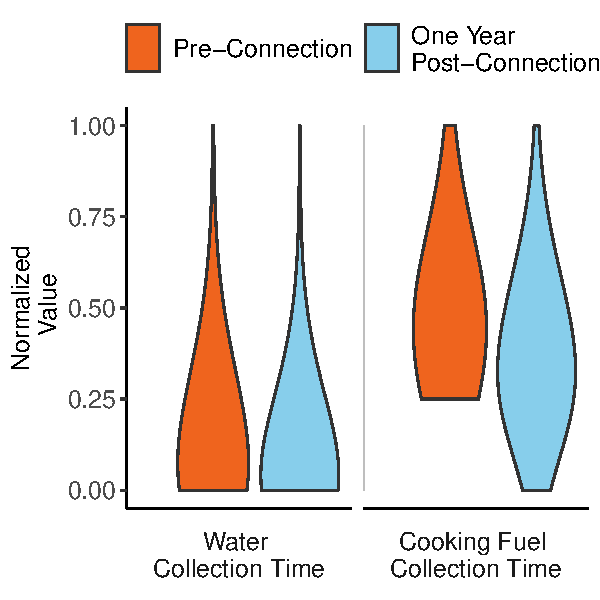
\includegraphics[width=\textwidth]{images/gender_equality_paired_results.pdf}
        \caption{Residents of newly electrified communities observed statistically significant declines in water and cooking fuel collection times.}
        \label{fig:gender_equality_paired_results}
    \end{subfigure}
    \hfill
    \begin{subfigure}[t]{0.48\textwidth}
        \centering
        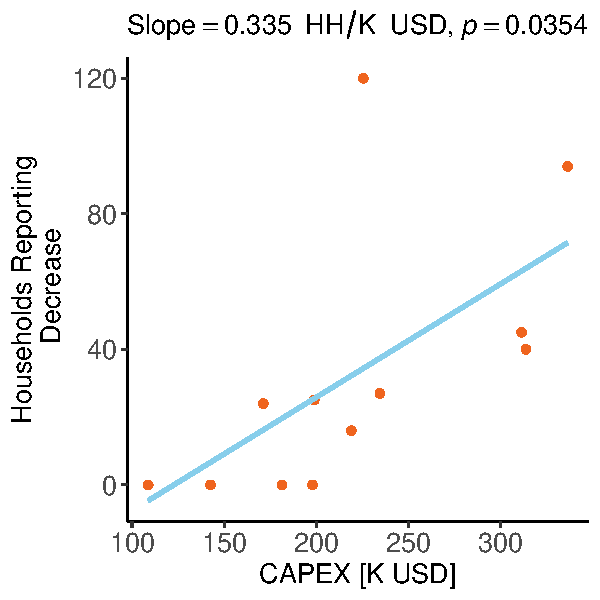
\includegraphics[width=\textwidth]{images/water_collection_time_regression_community.pdf}
        \caption{Increased CAPEX investment in mini-grids is correlated with ever-greater reductions in time spent collecting water.}
        \label{fig:water_collection}
    \end{subfigure}
    \caption{The presence of a mini-grid reduces the time residents have to spend on household chores.}
    \label{fig:water-and-fuel-collection}
\end{figure}

% collecting water and fuel
One reason behind the increase in school enrollment after connection to the mini-grid is that, in the pre-survey, 53.4\% of households reported delegating the responsibility of water collection to school-aged children. After connection to the mini-grid, only 15\% reported a similar answer in the post-survey. In the case of paired respondents, a comparable trend was noted, evidenced by a 29 percentage-point decrease in the proportion of households delegating water-fetching responsibilities to school-aged children. Overall, there was a $29\%\pm8\%$ decrease in the likelihood of school-aged children being tasked with this chore following the mini-grid installation.

As illustrated in \cref{fig:water-and-fuel-collection}, there was a notable reduction of $15\pm8$ hours spent collecting water and $36\pm10$ hours spent collecting cooking fuel per 100 households. An increase of 10 kWp in mini-grid PV capacity would lead to $25\pm22$ additional households reporting a decrease in water collection time, and an extra \$50,000 in CAPEX investment would result in an average of $15\pm15$ more households noting a similar improvement.

The proportion of households where men were involved in household chores, like collecting cooking fuel, rose from 10\% to 14\% between the pre-connection and post-connection surveys. However, this increase was less significant in the context of paired households, where the proportion only grew by 0.4 percentage points.

% new women jobs
\begin{figure}[t]
    \centering
    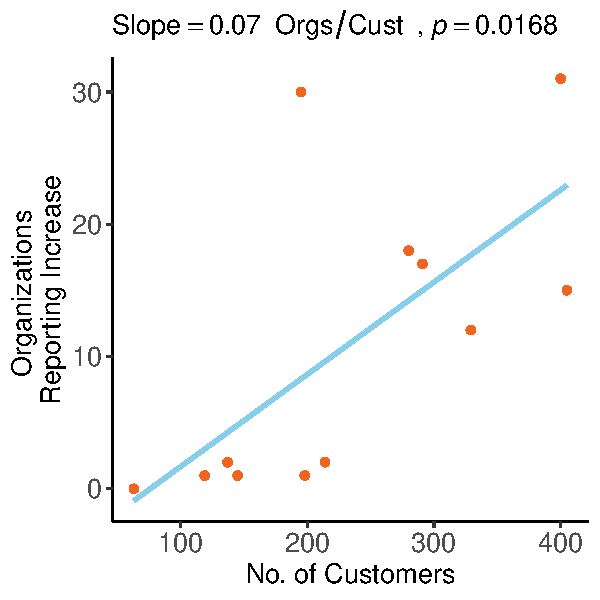
\includegraphics[width=0.5\textwidth]{images/hired_women_regression_community.pdf}
    \caption{For every ten additional customers connected to a mini-grid, approximately one more business would report hiring at least one more female employee.}
    \label{fig:women_employment}
\end{figure}

The analysis of economic opportunities for women involved two key questions directed at households and organizations focusing on business creation and job availability. Initially, 28\% of households reported having a woman-owned business, but this figure declined to 19\% post-connection. Among paired respondents, this represented a decrease of 4 percentage points. On the other hand, 17\% of the organizations surveyed reported employing at least one new female worker after the introduction of the mini-grid, marking a significant change in this aspect. As illustrated in \cref{fig:women_employment}, it was observed that connecting an additional 100 customers to the mini-grid would lead to $7\pm5$ more organizations employing at least one female worker.

\subsection{Productivity}
\begin{figure}[th]
    \centering
    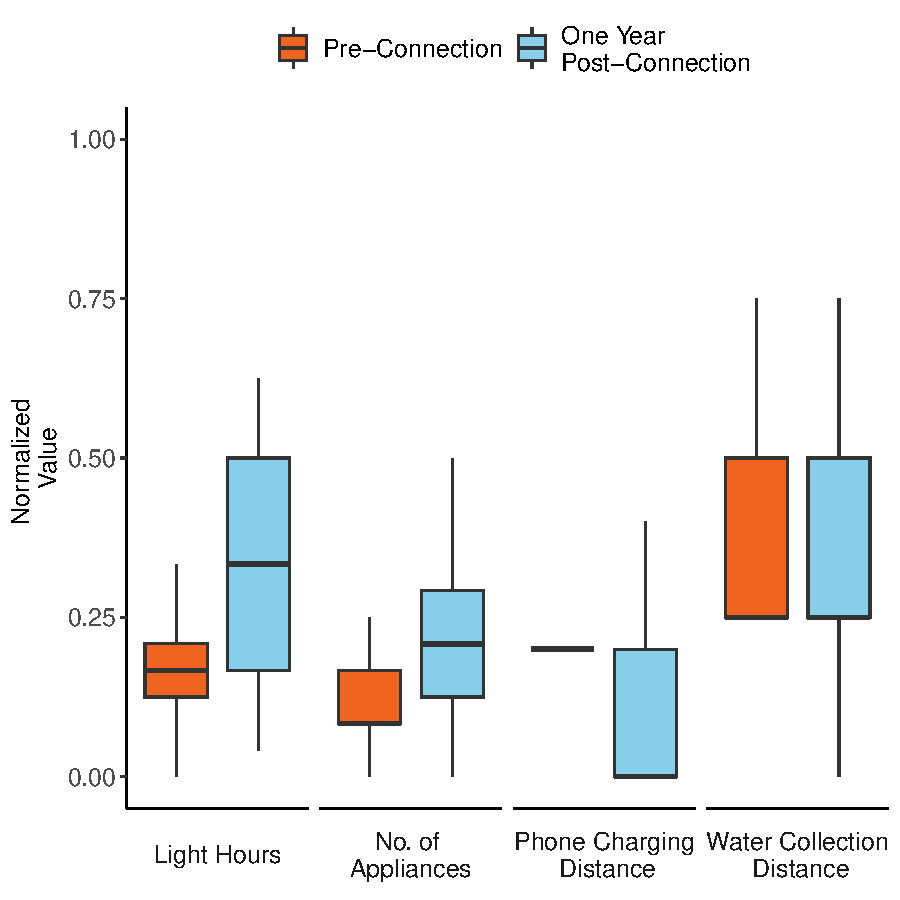
\includegraphics[width=0.7\textwidth]{images/productivity_paired_results.pdf}
    \caption{The installation of a new mini-grid had profound effects on community members' productivity, increasing the number of light hours and quantity of electrical appliances in the community while decreasing the distance required for members to charge their phones and collect water.}
    \label{fig:productivity_paired_results}
\end{figure}
The full results of the statistical analysis for questions pertaining to productivity are available in \cref{tab:app:productivity} in the appendix.

% Phone charging
As illustrated in \cref{fig:productivity_paired_results}, the installation of the mini-grid also had a notable impact on daily activities, with 58\% of respondents able to charge their phones every day and 94\% doing so at home, reducing the need to travel to neighbors, shops, or other locations for charging by a reported 66\%.

% Water and cooking fuel collection
Regarding water and cooking fuel collection time, there was a marked improvement in efficiency post-connection to the mini-grid. In the post-survey, 66\% of respondents reported that it took them less than one hour to collect water, a significant increase from the 57\% who said the same in the initial survey. This increase was also reflected in the paired sample, where an 18 percentage-point change in proportions was observed. Similarly, the time spent collecting cooking fuel decreased notably. In the post-survey, 63\% of respondents indicated that this task took less than one hour, a substantial improvement from the initial survey, where only 35\% reported such efficiency.

\begin{figure}[th]
    \centering
    \begin{subfigure}[t]{0.48\textwidth}
        \centering
        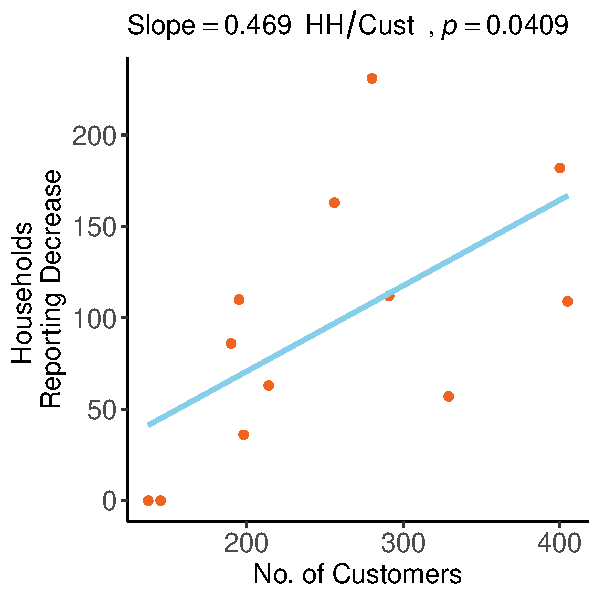
\includegraphics[width=\textwidth]{images/power_sources_unclean_regression_community.pdf}
        \caption{Almost half of all additional community members connected to a mini-grid are statistically likely to reduce or eliminate their usage of unclean power sources such as diesel, petrol, and kerosene.}
        \label{fig:unclean_power_usage}
    \end{subfigure}
    \hfill
    \begin{subfigure}[t]{0.48\textwidth}
        \centering
        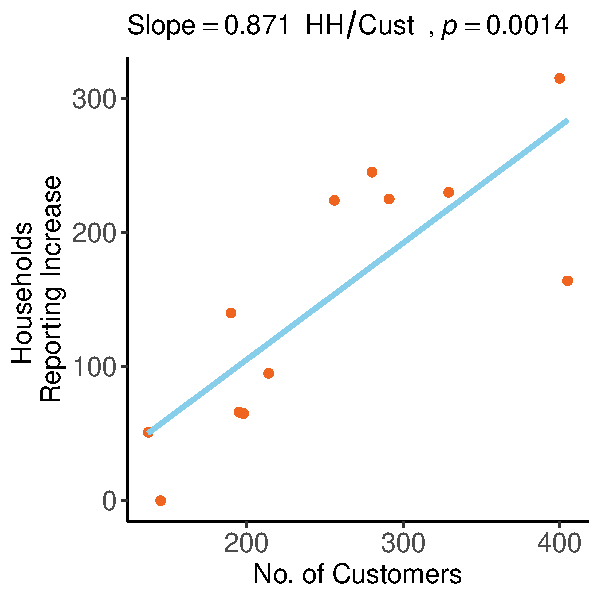
\includegraphics[width=\textwidth]{images/appliances_count_regression_community.pdf}
        \caption{Almost nine out of every ten additional community members connected to a mini-grid are statistically likely to buy new appliances to take full advantage of their new source of electricity.}
        \label{fig:appliances}
    \end{subfigure}
    \caption{Upon connecting to a mini-grid, community members quickly transition from using unclean power sources like diesel, petrol, and kerosene to utilizing this cleaner, cheaper energy option for powering their electrical appliances.}
    \label{fig:appliances-and-unclean-power}
\end{figure}

% Power sources
Prior to connecting to the mini-grid, a majority of the households had limited or no reliable power sources. Specifically, 55\% of households depended on petrol generators. However, one year after the mini-grid connection, this number dramatically decreased to just 1\%, with the mini-grid becoming the primary power source for 91\% of survey respondents. The shift was also evident in the broader reduction of unclean energy sources, including diesel, petrol, and kerosene, which decreased from 66\% in the pre-survey to 19\% in the post-survey. Among paired households, this represented a 7 percentage-point reduction. As illustrated in \cref{fig:unclean_power_usage}, every 100 additional customers connected onto the mini-grid would result in $47\pm45$ fewer households using unclean power sources.

% Light hours and new appliances
Post-connection, households reported significant improvements in their energy access: an average of seven hours of lighting per day and the use of an average of four electronic devices, compared to only four hours of lighting and two appliances before connection. Moreover, 55\% of households acquired new appliances since connecting to the mini-grid. As illustrated in \cref{fig:appliances-and-unclean-power}, for every 100 additional customers connected to the mini-grid, $87\pm45$ acquired new appliances.

% School performance
\begin{figure}[th]
    \centering
    \begin{subfigure}[t]{0.48\textwidth}
        \centering
        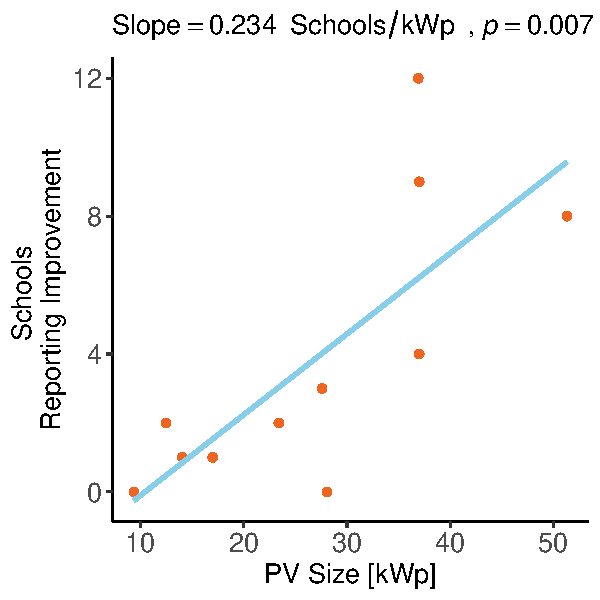
\includegraphics[width=\textwidth]{images/school_performance_regression_community.pdf}
        \caption{Additional mini-grid solar array capacity resulted in more schools reporting improvements in children's academics.}
        \label{fig:academics_schools}
    \end{subfigure}
    \hfill
    \begin{subfigure}[t]{0.48\textwidth}
        \centering
        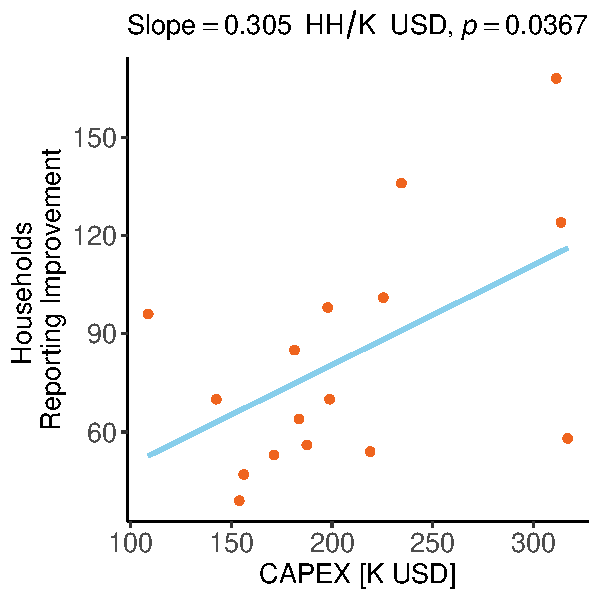
\includegraphics[width=\textwidth]{images/school_performance_change_regression_community.pdf}
        \caption{Every additional \$50,000 in CAPEX investment into the mini-grid led to approximately 15 more households reporting an improvement in their kids' academics.}
        \label{fig:academics_households}
    \end{subfigure}
    \caption{Educators and parents both report that larger mini-grids lead to more well-educated students.}
    \label{fig:academic-performance}
\end{figure}

With the connection to the mini-grid providing a more reliable source of power, there were extended lighting hours for both schools and households, directly benefiting school-aged children. In this context, both households and schools were surveyed about changes in academic performance following the mini-grid installation. The results, illustrated in \cref{fig:academic-performance}, were telling: 46\% of households observed a positive change in the academic performance of their children, while a significant 92\% of schools reported similar improvements. Connecting an additional 100 customers to the mini-grid would lead to $19\pm17$ more households observing an improvement in the children's academics. Similarly, an investment of an additional \$50,000 in CAPEX is associated with $15\pm15$ more households reporting a comparable improvement. Furthermore, an increase of 10 kWp in the mini-grid capacity would result in $2\pm2$ more schools noting such an improvement in academic performance.

% C&I
\begin{figure}[th]
    \centering
    \begin{subfigure}[t]{0.48\textwidth}
        \centering
        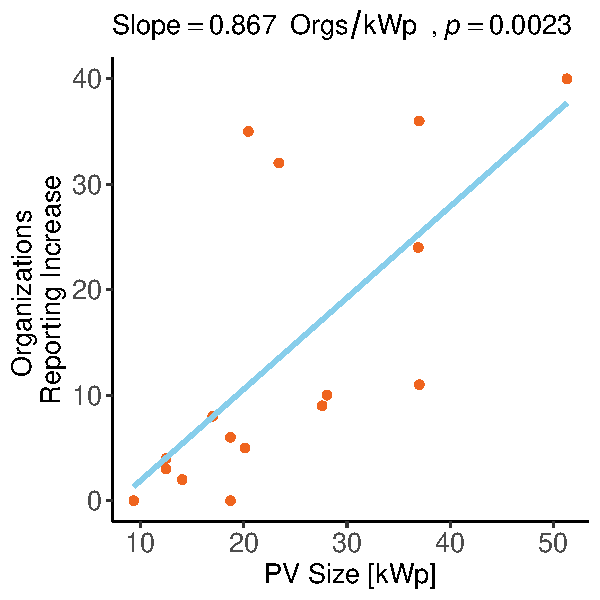
\includegraphics[width=\textwidth]{images/ci_offering_change_regression_community.pdf}
        \caption{Additional mini-grid solar array capacity resulted in more product or service offerings.}
        \label{fig:ci_offering}
    \end{subfigure}
    \hfill
    \begin{subfigure}[t]{0.48\textwidth}
        \centering
        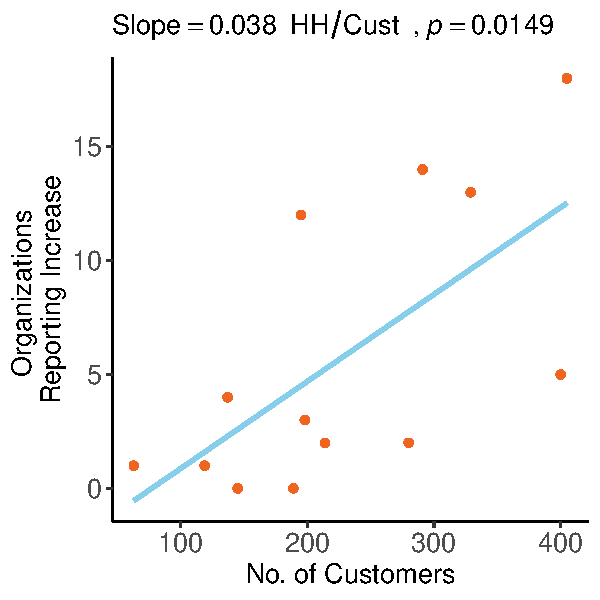
\includegraphics[width=\textwidth]{images/workforce_change_regression_community.pdf}
        \caption{Every additional 100 customer connections led to approximately 4 more establishments hiring at least one more worker.}
        \label{fig:workforce_change}
    \end{subfigure}
    \caption{Establishments reporting an increase in their workforce and offerings.}
    \label{fig:ci_productivity}
\end{figure}

Among commercial and institutional customers connected to the mini-grid, a substantial 87\% reported an increase in their operational hours. Among all establishments, 16\% of them have recruited new employees, while 51\% have broadened their range of products and services. As illustrated by \cref{fig:ci_productivity}, an increase of 10 kWp in the mini-grid capacity is associated with $9\pm5$ more organizations reporting an expansion in their product or service offerings, and every additional 100 customer connections correlates with $4\pm3$ more organizations employing at least one new worker. 

\subsection{Health}
The full results of the statistical analysis for questions pertaining to health are available in \cref{tab:app:health} in the appendix.

% Clinic electricity
Local health clinics in newly electrified communities benefited greatly from access to power from their mini-grids. The access to electricity in clinics showed a significant improvement in the post-survey, with 82\% of respondents indicating that the nearest clinic had electricity, a considerable increase from only 35\% in the initial survey. This positive shift was also evident in the paired sample, where an increase of 53 percentage points was observed. One way in which clinics utilized electricity was to provide refrigeration, enabling the safe storage of vaccines, medications, and blood supplies: 86\% of post-survey responses confirmed refrigeration availability, up from 41\% initially, translating to a 48 percentage-point improvement in the paired sample. Among all the clinics surveyed, 79\% reported the addition or enhancement of at least one service they provide, with a median of three services being improved or added.

\begin{figure}[t]
    \centering
    \begin{subfigure}[t]{0.48\textwidth}
        \centering
        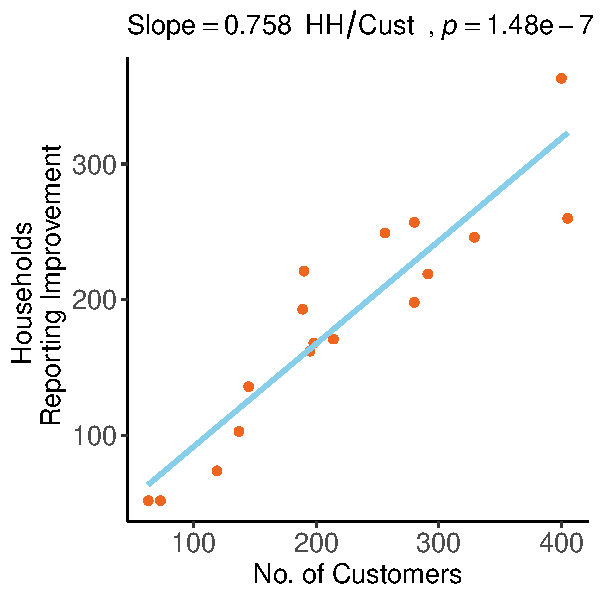
\includegraphics[width=\textwidth]{images/better_access_health_minigrid_regression_community.pdf}
        \caption{For every four additional customers connected to a mini-grid, approximately three of which will be households, all three will likely report an improvement in the quality of healthcare in their community.}
        \label{fig:better_healthcare}
    \end{subfigure}
    \hfill
    \begin{subfigure}[t]{0.48\textwidth}
        \centering
        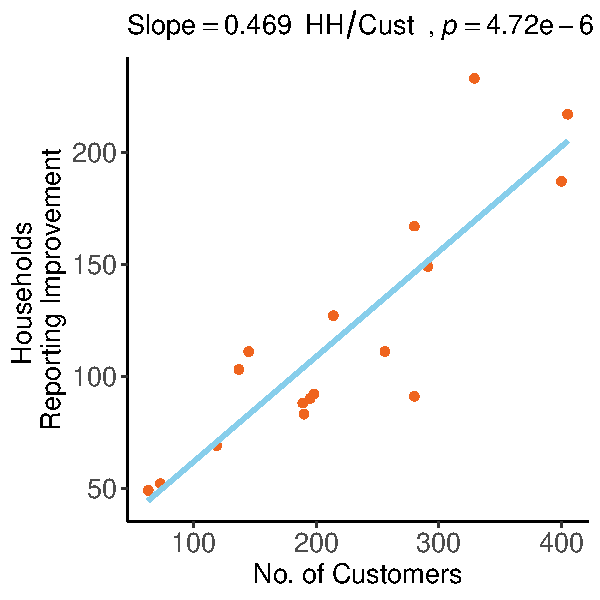
\includegraphics[width=\textwidth]{images/minigrid_access_life_improvement_regression_community.pdf}
        \caption{For every four additional customers connected to a mini-grid, two households in the community will likely report an improvement in their overall quality of life.}
        \label{fig:life_improvement}
    \end{subfigure}
    \caption{Connecting additional customers to a mini-grid significantly enhances a community's perceived well-being.}
    \label{fig:well_being}
\end{figure}

Electrification of clinics significantly influenced community members' views on their health. Following the mini-grid installation, 58\% of respondents reported an enhancement in their lives owing to improved healthcare facilities. The connection of an additional 100 customers to a mini-grid results in an average of $76\pm18$ more households reporting access to better healthcare. Furthermore, it leads to approximately $47\pm14$ more households reporting an overall enhancement in their quality of life. These effects are illustrated in \cref{fig:well_being}.

% kerosene lamps
\begin{figure}[th]
    \centering
    \begin{subfigure}[t]{0.48\textwidth}
        \centering
        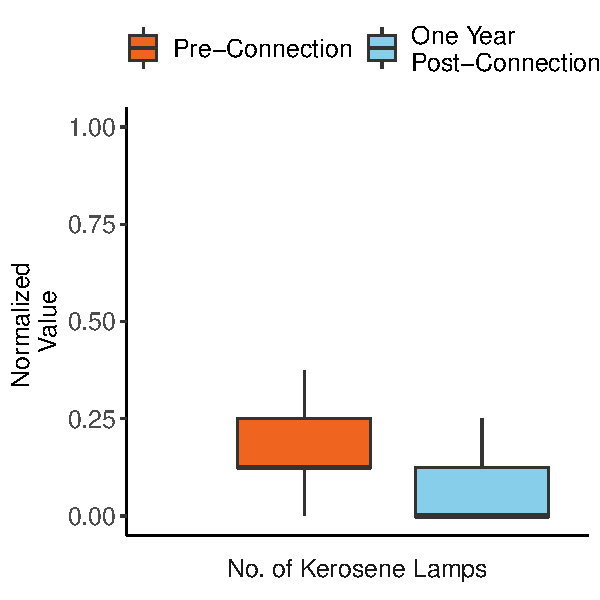
\includegraphics[width=\textwidth]{images/health_paired_results.pdf}
        \caption{The median household used one kerosene lamp before the mini-grid connection, and none one year after connection.}
        \label{fig:paired-kerosene}
    \end{subfigure}
    \hfill
    \begin{subfigure}[t]{0.48\textwidth}
        \centering
        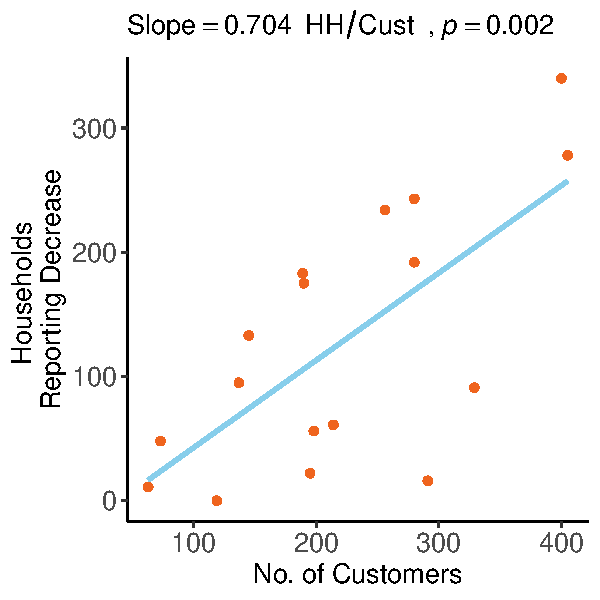
\includegraphics[width=\textwidth]{images/kerosene_lamp_usage_change_regression_community.pdf}
        \caption{For every ten new customer connections, of which eight will likely be households, seven of those households will likely decrease their reliance on kerosene.}
        \label{fig:regression-kerosene}
    \end{subfigure}
    \caption{Community kerosene consumption decreases significantly after the installation of a new mini-grid.}
    \label{fig:kerosene}
\end{figure}
Connecting 100 additional households to the mini-grid is expected to result in a significant reduction in the use of kerosene lamps: connecting 100 households results in $36\pm20$ fewer kerosene lamps used. \cref{fig:kerosene} illustrates the profound effect of mini-grids on reducing kerosene usage. Put simply, the median household used one kerosene lamp before the mini-grid connection, and none one year after connection.

% Water
The transition to the mini-grid has led to notable improvements in water quality for the surveyed communities. There was a decrease in the use of dirty water, with pre-survey respondents reporting a 38\% usage rate, which dropped to just 15\% in the post-survey. Concurrently, the majority of households shifted to using community wells or pumps, accounting for 50\% of the water sources post-connection.

When specifically asked about access to clean drinking water, 61\% of post-survey respondents confirmed having such access, a significant rise from 36\% in the initial survey. In the paired samples, this represented a positive increase of 12 percentage points. The primary source of this clean drinking water shifted dramatically, with 60\% of post-survey respondents sourcing it from the community, up from 22\% initially. This shift also led to a reduced reliance on boiling water for purification, which decreased from 41\% to 23\%. One year after connection to a mini-grid, households were 1.9 times more likely to have access to clean drinking water.

\subsection{Safety}
The full results of the statistical analysis for questions pertaining to safety are available in \cref{tab:app:safety} in the appendix.

Although there was no statistically significant change in the overall number of respondents who reported feeling safe in their communities, statistically significant shifts were observed in the reasons cited by those who felt unsafe. The perceived threat from potential theft saw a significant increase, rising from 31\% pre-connection to 73\% one year after connection. Conversely, concerns related to the lack of community lighting decreased substantially from 40\% to 17\%, and the lack of safety due to unsafe travel dropped from 23\% to 7\%. This change is partly attributed to the improvement in community lighting, with 56\% of respondents acknowledging its presence post-connection, a considerable increase from just 22\% pre-connection. This represents a 13 percentage-point increase in the paired sample proportions.

Household lighting saw improvement, with exterior lights increasing from 21\% to 58\% of households post-connection, and 68\% being powered by the mini-grid.

\subsection{Economic Activity}
The full results of the statistical analysis for questions pertaining to economic activity are available in \cref{tab:app:econ} in the appendix.

% Business owner in the household
Following the mini-grid installation, there was a noticeable shift in the occupational dynamics within households. Specifically, 20\% of households reported a change in the occupation of the primary income provider during the first year after connection to the mini-grid. Part of this is due to a discernible increase in entrepreneurial activity. Post-mini-grid installation, 73\% of households confirmed having a business owner in the household, a rise from 70\% observed initially. Notably, 19\% of these households reported that the business was established immediately following the mini-grid installation. This represents a 10 percentage-point increase in business ownership within the paired sample.

% \begin{figure}[t]
%     \centering
%     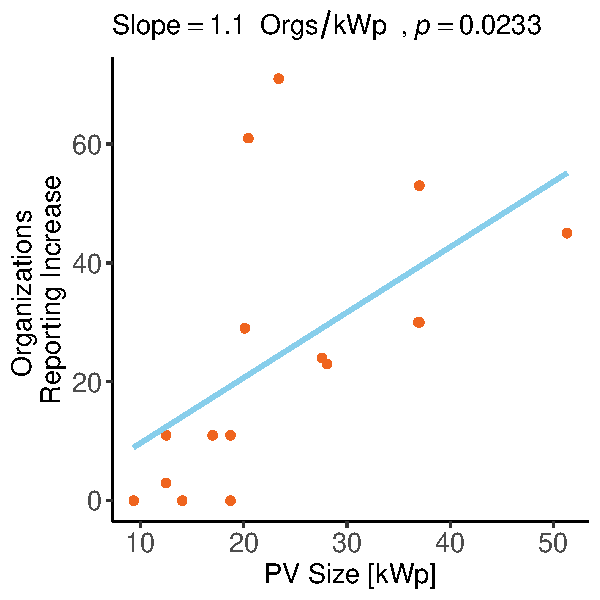
\includegraphics[width=0.5\textwidth]{images/earnings_change_regression_community.pdf}
%     \caption{Every additional 10 kWp of installed solar panels correlated with six local businesses reporting increased earnings.}
%     \label{fig:earnings_change}
% \end{figure}

% Org earnings
\begin{figure}[t]
    \centering
    \begin{subfigure}[t]{0.48\textwidth}
        \centering
        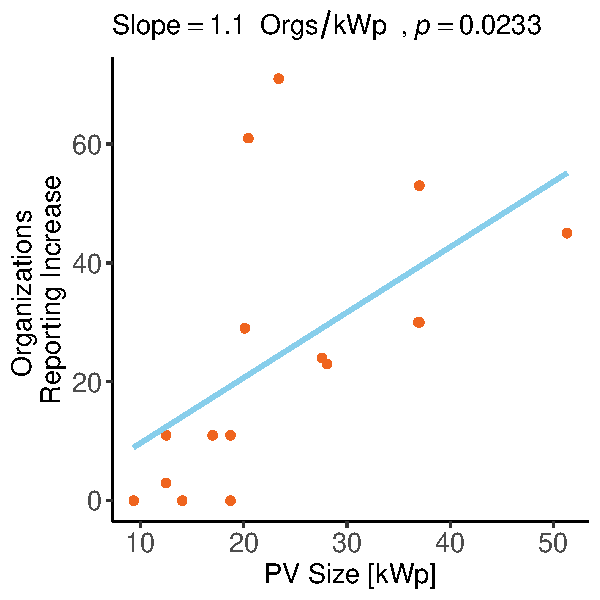
\includegraphics[width=\textwidth]{images/earnings_change_regression_community.pdf}
        \caption{Every additional 10 kWp of installed solar panels correlated with six local businesses reporting increased earnings.}
        \label{fig:earnings_change}
    \end{subfigure}
    \hfill
    \begin{subfigure}[t]{0.48\textwidth}
        \centering
        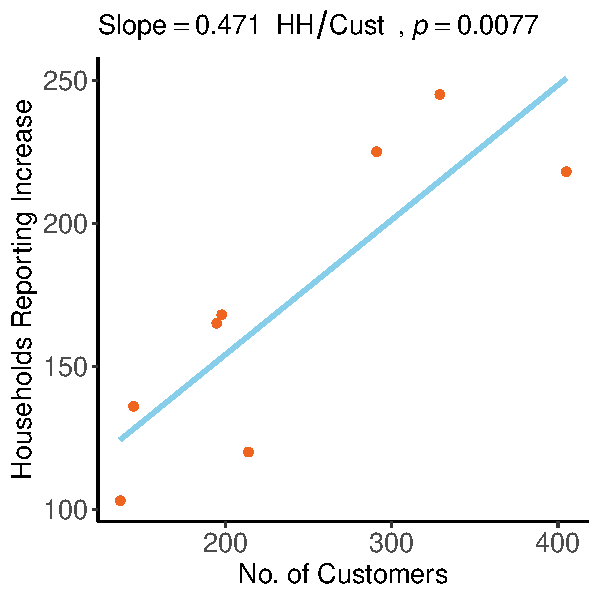
\includegraphics[width=\textwidth]{images/kenya_avg_household_income_regression_community.pdf}
        \caption{For every ten new customer connections in Kenya, of which eight will likely be households, five of those households will likely experience an increase in their average monthly income in Kenyan Shillings.}
        \label{fig:kenya_incomes}
    \end{subfigure}
    \caption{Earnings and Kenyan Monthly Incomes increased significantly after the installation of a new mini-grid.}
    \label{fig:economic_improvement}
\end{figure}
Among the commercial and institutional customers surveyed, a substantial 85\% reported an increase in their overall earnings following the mini-grid installation. As illustrated in \cref{fig:economic_improvement}, for every additional 10 kWp in mini-grid capacity, there is an increase of $6\pm4$ organizations reporting a boost in their earnings. 
%Similarly, an extra CAPEX investment of \$50,000 is associated with $5\pm5$ more organizations reporting an improvement in earnings. 

% Income
In Kenya, the median monthly income in the communities rose from 5,000 to 6,000 Kenyan Shillings (KES) post-connection, while in Nigeria, the median household income actually decreased from 47,500 to 25,000 Nigerian Naira (NGN) after the mini-grid connection. Notably, 24\% of Kenyan households reported a positive increase in their incomes, compared to 18\% of Nigerian households. Among the paired respondents, the income change was significant: in Nigeria, there was a decrease of $24,079\pm4,496$ NGN, whereas in Kenya, there was an increase of $13,037\pm1,662$ KES. Every 10 additional customer connections in Kenya is correlated with $5\pm3$ more households reporting an increase in their average household income.

% Cost of phone charging, cooking energy, and kerosene lamps
\begin{figure}[t]
    \centering
    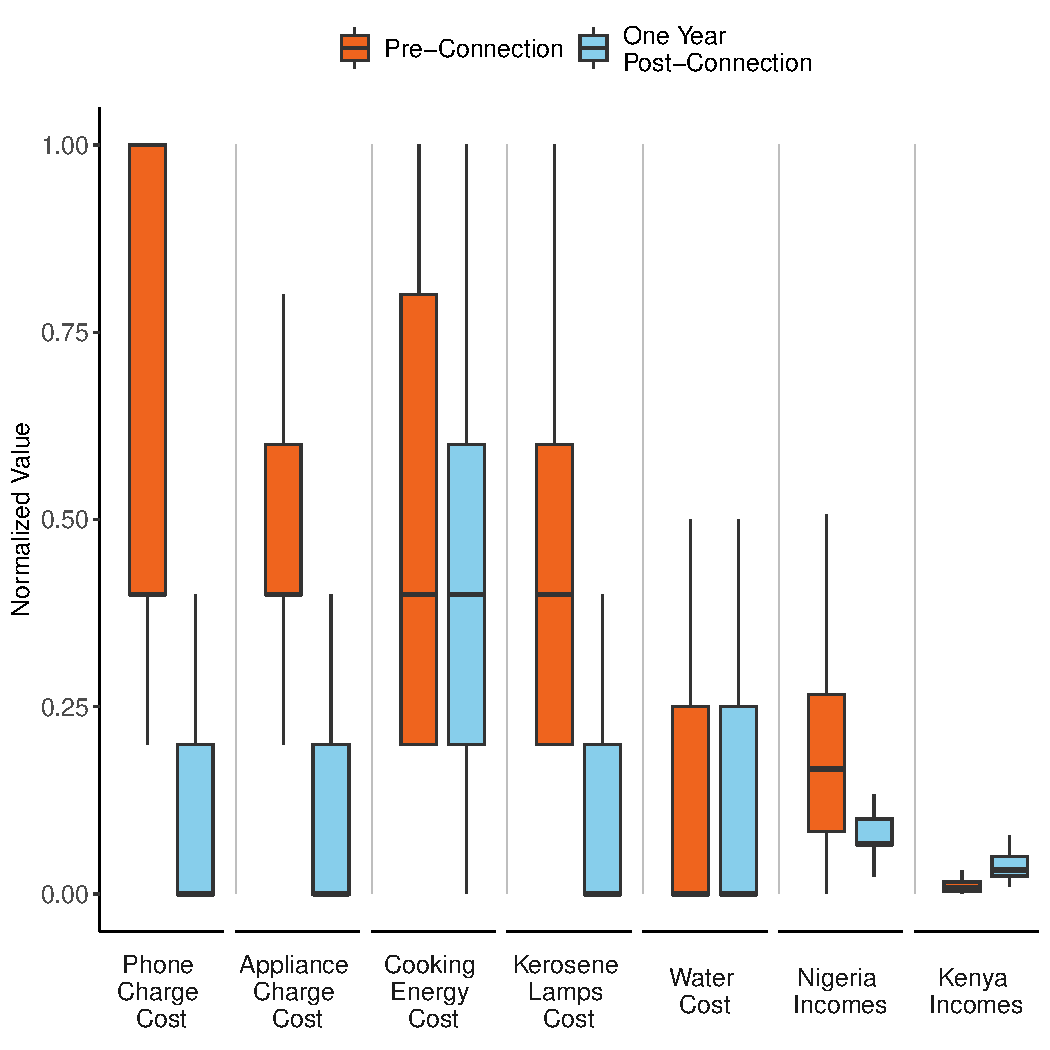
\includegraphics[width=0.9\textwidth]{images/economic_activity_paired_results.pdf}
    \caption{Installing a mini-grid in a community reduced the cost of phone and appliance charging, cooking energy, kerosene lamps, and water.}
    \label{fig:economic_paired_results}
\end{figure}

% Water Cost
As illustrated in \cref{fig:economic_paired_results}, before the mini-grid installation, 18\% of Nigerian households spent between 0 and 5,000 NGN monthly on water. Post-installation, 90\% of respondents indicated zero water costs, instead getting all their water from community wells, marking a 94 percentage-point increase in those not paying anything and a substantial decrease of 3,000 NGN per household for water costs. For every 10 customer connections in Nigeria, $2\pm2$ more households would report a decrease in water cost. In Kenya, prior to connection, 74\% of households spent between 0 and 3,000 KES monthly on water, and 27\% paid 5,000 KES or more. After connection, 57\% of households reported no water expenses.

% Phone Charging Cost
Before connecting to the mini-grid, 84\% of Nigerian households were spending between 0 and 1,000 NGN monthly to charge their phones due to the absence of electricity. Post-connection, a significant reduction in this expense occurred, with 96\% of post-survey respondents reporting no additional costs beyond their household power bill. In the paired sample, this equates to a 97 percentage-point increase in those not paying for phone charging and a marked decrease of $900\pm100$ NGN per household each month. For every additional 10 customer connections in Nigeria, $7\pm4$ more households would report a decrease in phone charging cost. In Kenya, pre-connection, 43\% of households spent between 0 and 750 KES monthly on phone charging, and 55.5\% paid 1,000 KES or more. After connection, a considerable number of households saw this cost alleviated, with 45\% of post-connection respondents indicating no extra expenses beyond their household power bill. In the paired sample, this translates to a 15 percentage-point increase in those not incurring phone charging costs and a significant monthly reduction of 100 KES per household.

% Appliance Charging Cost
Initially, 84\% of Nigerian households incurred costs between 0 and 6,000 NGN monthly for appliance charging due to unreliable power sources. However, one year after connecting to the mini-grid, 93\% of respondents no longer faced any additional charging costs. In the paired sample, there was a 94 percentage-point increase in households reporting no appliance charging costs and a significant monthly reduction of 3,000 NGN per household. In Kenya, 99\% of households initially spent between 0 and 4,000 KES monthly to charge appliances. A year after mini-grid connection, 37\% of households reported no longer having this expense. The paired sample showed a 13 percentage-point increase in those not paying for appliance charging and a notable decrease of 150 KES per household each month.

% Cooking Energy Cost
In Nigeria, before the mini-grid installation, 84\% of respondents spent between 0 and 3,000 NGN monthly on cooking energy. One year after installation, 34\% reported their cooking costs had fallen to between 0 and 1,000 NGN, a significant increase from 14\% pre-connection. In the paired sample, this shift represented a 26 percentage-point increase in those with a lower cooking energy bill in the 0 to 1,000 NGN range, alongside a notable monthly decrease in cooking energy costs of 1,500 NGN per household. In Kenya, prior to the mini-grid connection, 96\% of households were spending between 0 and 2,000 KES monthly on cooking energy. Post-connection, a cost reduction was observed, with 79\% now paying either nothing or between 0 and 1,500 KES. The paired sample analysis showed a 4 percentage-point increase in households paying nothing, a 27 percentage-point decrease in those spending between 0 and 1,000 KES, and a 17 percentage-point increase in those now spending between 1,000 and 1,500 KES on cooking energy.

% Kerosene Lamps Cost
Prior to the mini-grid connection, 57\% of Nigerian households were spending between 0 and 1,400 NGN monthly on expenses related to kerosene lamps. A year after connection, a significant change was observed: 91\% of post-survey respondents reported no expenditure on kerosene. In the paired sample, this equated to an 89 percentage-point increase in households no longer incurring costs for kerosene lamps, with a substantial monthly reduction of $1,000\pm400$ NGN per household. For every additional 10 customer connections in Nigeria, $6\pm2$ more households would report a decrease in the amount spent on kerosene lamps. In Kenya, initially, 98\% of households spent between 0 and 1,000 KES on kerosene lamp-related costs. After a year of mini-grid connectivity, 72\% of respondents reported eliminating these expenses. This change represented a 47 percentage-point increase in the paired sample for those not needing to spend on kerosene lamps, and a notable monthly decrease of 200 KES per household.